\chapter{Query Processing}
In this chapter we will introduce how to answer queries such as “stanford university” as a phrase and 
thus the sentence “I went at Stanford my university” is not a match.

The first approach consist to use the \emph{$2$-word indexes}, so for example the text "Friends, Romans, Countrymen" would generate the biwords
friends romans and romans countrymen, so each of these $2-$words is now an entry in the dictionary and the two-word phrase query-processing is immediate.

Longer phrases are processed by reducing them to bi-word queries in AND, so "stanford university palo alto"
can be broken into the Boolean query on biwords, such as "stanford university AND university palo AND palo alto".\newline
The problem of this approach is that need the docs to verify, can have false positives and index blows up, so a better approach consist to \emph{positional indexes},
where in the postings we store for each term and  document the position(s) in which occurs; typically queries happens with free text,
so just a set of terms typed into the query box common on the web and users prefer docs in which query terms
occur within close proximity of each other so we would like scoring function to take this into account.

With positional index size we can compress position values/offsets and nevertheless, a positional index expands
postings storage by a factor $2$-$4$ in English, it is now commonly used because of the power and usefulness of phrase and proximity queries, 
and we introduce now the \emph{Soft-AND}, used to solve phrase query, which algorithm is visible in figure \ref{img:softAnd}.

\begin{figure}
	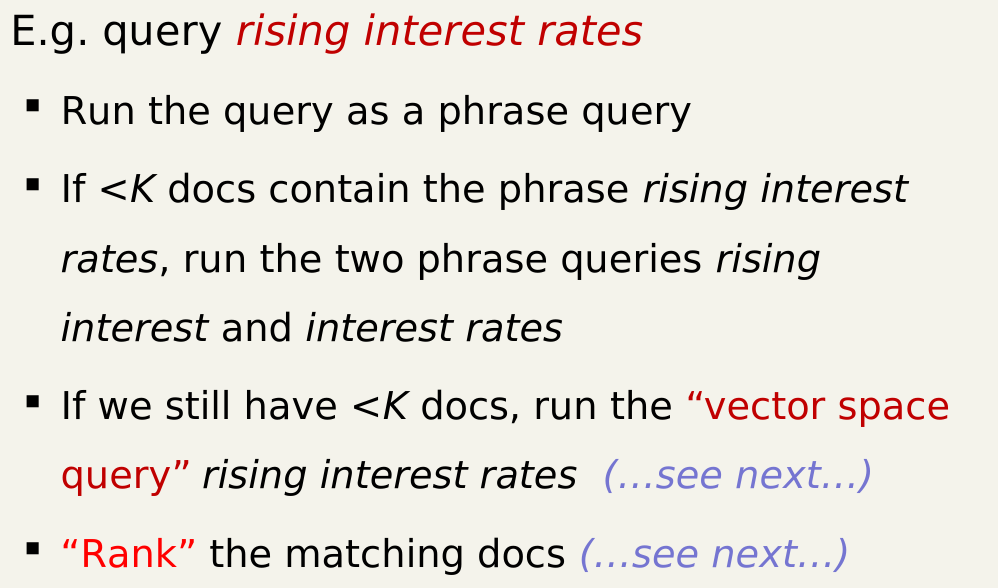
\includegraphics[width=\textwidth]{Images/softAnd}
	\caption{SoftAnd Algorithm procedure}
	\label{img:softAnd}
\end{figure}
To achieve better results we cache and there are two opposite approaches:
\begin{enumerate}
	\item Cache the query results and exploits query locality.
	\item Cache pages of posting lists and so exploits term locality.
\end{enumerate}
In figure \ref{img:cacheQuery} is possible to note how consist the cache for query and/or postings.

\begin{figure}
	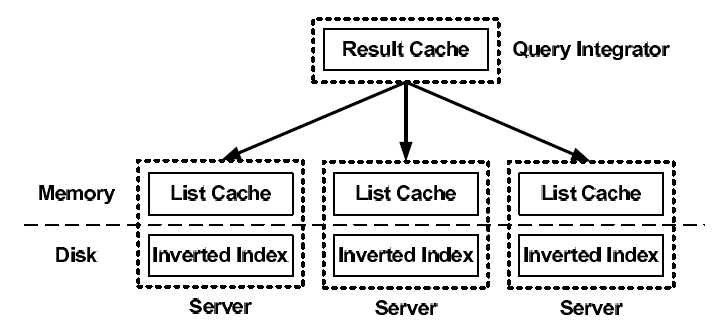
\includegraphics[width=\textwidth]{Images/cacheQuery}
	\caption{Composition of Cache on Query/Postings}
	\label{img:cacheQuery}
\end{figure}
To have faster query we can use \emph{tiered query}, where we break postings up into a hierarchy of lists, so inverted index thus broken up into tiers of
decreasing importance and at query time we use top tier unless it fails to yield $K$ docs and if so drop to lower tiers, as we can note in figure \ref{img:tiered}.

\begin{figure}
		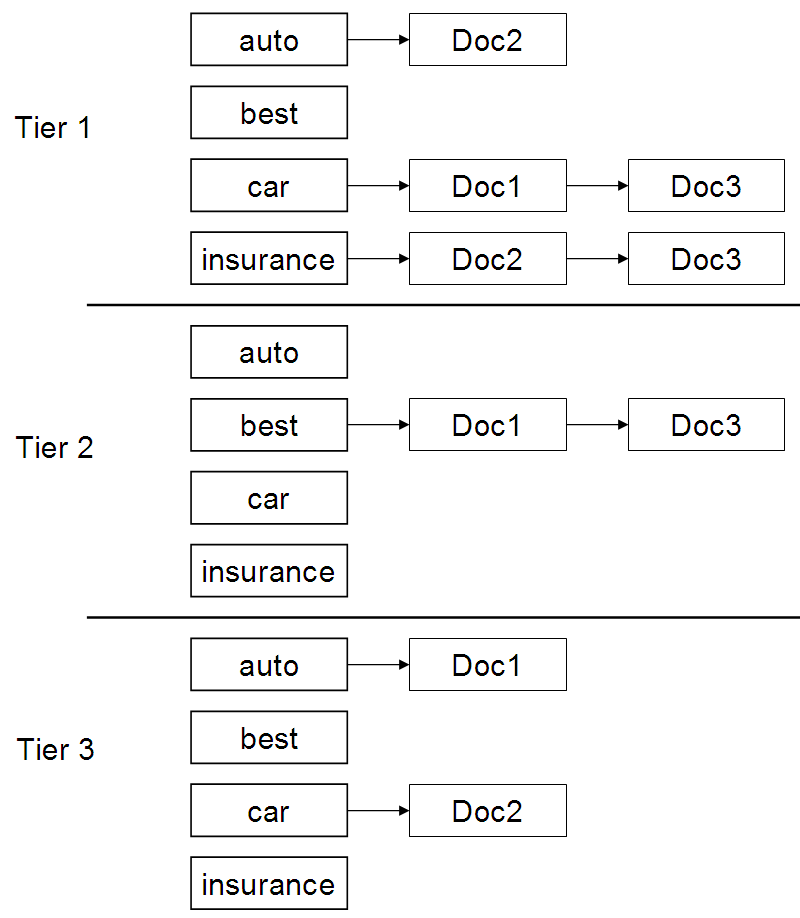
\includegraphics[width=0.7\textwidth]{Images/tieredIndex}
	\caption{Example of Tiered Queries}
	\label{img:tiered}
\end{figure}


